    \chapter{INTRODUCTION}
\label{chp:introduction}

The autonomous vehicle market is experiencing rapid expansion, with numerous established brands and startups dedicating considerable efforts, resources, and investments to secure a position in this lucrative sector that may create 300\$ billion to 400\$ billion in revenues by the year 2035 \cite{McKinsey2023}. These companies strive to offer sustainable, technologically advanced solutions that enhance user experience and provide innovative advancements. In recent years, there has been a proliferation of essential technologies that have greatly facilitated the advancement and reliable operation of autonomous vehicles, including the availability of large-scale data analytics (commonly known as big data), increased computational capabilities, and a wide range of sensor technologies such as ultrasonic sensors, \gls{radar}, \gls{lidar}, cameras, and the integration of all these sensors through sensor fusion techniques \cite{Hussain2018}.

According to the \gls{sae}, autonomous vehicles can be classified into six levels based on their ability to operate without human intervention. Level 0 represents vehicles that rely entirely on human drivers for all aspects of driving. Level 1 vehicles have certain functions automated, such as braking or steering, but still require full driver engagement. At Level 2, the automation system can control both steering and acceleration/deceleration, while the driver must remain fully attentive and ready to take control when needed. Level 3 vehicles can operate autonomously under certain conditions, allowing the driver to engage in other tasks, but prompt transition is required if the system requests intervention. Level 4 vehicles are highly autonomous and can operate without human input in specific geographic areas or predetermined scenarios, but not in all conditions. Finally, Level 5 vehicles are fully autonomous and can operate under all conditions, without the need for human intervention, enabling passengers to engage in non-driving related activities \cite{SAE2021}.

Much like a human driver relies on their sight, touch, and hearing to navigate and make informed decisions on the road, autonomous vehicles have primarily focused on vision and touch, neglecting the crucial sense of hearing or audition. This omission is akin to a human driver being deprived of their ability to hear, which would severely limit their situational awareness and pose significant challenges in detecting important auditory cues, such as emergency vehicle sirens, approaching vehicles or any other road users.

In the realm of human perception, the ability to effortlessly segregate and identify individual sound sources within a complex acoustic mixture is a common phenomenon, for instance, an individual can effortlessly pick out a specific voice amidst a bustling background that includes the voices of other individuals and music. The field of sound analysis, commonly referred to in the literature as \gls{casa} \cite{Hermes2023}, delves into the investigation of methods to disentangle and recognize sound sources present in an auditory scene with the primary objective to equip computers with the ability to perceive and comprehend audio content, akin to the human auditory system. 

Given the vast scope of \gls{casa} applications, this field of research is typically subdivided into three core areas according to \textcite{Wang2006}:

\begin{itemize}
    \item \textbf{Context awareness}, also known as audio context recognition, pertains to identifying the location or ongoing activity within a specific environment based on audio information or events. It provides a context location of the sound, such as determining whether it's coming from a supermarket or a highway;
    \item \textbf{Sound event detection and recognition} involves categorizing individual sound events present in an auditory scene. It addresses the question of "who and what" by recognizing the specific sound sources within the scene, for example a children crying;
    \item \textbf{General audio classification} involves classifying and recognizing the contents of audio signals, commonly utilized for audio content retrieval, indexing, and audio-based searching.  
\end{itemize}

Understanding the acoustic environment by \textbf{detecting and recognizing sound events} can be crucial for autonomous vehicles to perceive and react to their surroundings, providing a more comprehensive sensory system for safer and more efficient autonomous driving. By deploying audio classification algorithms on embedded systems within these vehicles, real-time \gls{esr} can be achieved, allowing for advanced functionalities such as emergency vehicle detection, sound-based traffic monitoring, and early warning systems. Moreover, the effective utilization of embedded systems can alleviate the burden on external computing infrastructure and facilitate seamless integration of \gls{esr} into the existing vehicle architecture.


There is a substantial body of literature covering \gls{esr} algorithms that are implemented on embedded devices, operating at both low-level platforms such as microcontrollers \cite{Abreha2014} and \cite{Nordby2019}, as well as high-level platforms like \gls{fpga} and \gls{tpu} \cite{Silva2019}, \cite{Vandendriessche2021} and \cite{Lhoest2021}. Despite the lack of research focusing on the application of these algorithms in autonomous vehicles or regular passenger vehicles, there is significant potential for research and development in this area. By addressing this research gap, the overall performance and safety of autonomous and regular passenger vehicles can be improved, while also making valuable contributions to the emerging field of acoustic perception in intelligent transportation systems. In addition to the identified research gap, it is worth noting that the field of acoustic perception in intelligent transportation systems has already attracted attention in the industry. Google Inc., for instance, has filed a patent related to the utilization of audio data for controlling autonomous vehicles \cite{Ferguson2014}.


\section{CONTEXT}
\label{sec:introduction_context}

Urban mobility is a complex interaction of energy usage, movement patterns, and spatial allocation, and particularly in densely populated cities, space is a scarce and highly valuable resource. The extent and design of available space determine individuals' abilities to accomplish their professional and personal objectives, reconcile their desires and necessities, and enhance the quality of their living and working conditions. An alternative to achieving these goals relies on urban centers being planned with reduced vehicle presence, decreased parking infrastructure, and minimized environmental pollution. Furthermore, the integration of previously distinct and individual mobility systems is necessary to create a cohesive and efficient urban mobility network.

The concept of "SmartCity" has emerged as a response to the global phenomenon of urbanization and the projected growth of cities. This overarching term, embraced by politics, business, administration, and urban planning, encapsulates comprehensive development strategies aimed at enhancing efficiency, technological advancement, sustainability, and inclusivity within cities, primarily concentrate on technical, economic, and social innovations\footnote{Citations were omitted due to the disclaimed blocking and restriction notice.}.

To fulfill the objectives of SmartCity endeavors, certain technical and urban planning prerequisites need to be addressed, namely a few of them:

\begin{itemize}
    \item Establishing designated areas for new mobility concepts where only bicycles are allowed, prohibiting individual or private vehicles. Pedestrians should always have priority over other vehicles, and designated pedestrian crossings may not be necessary;
    \item Integrating public transportation into the urban mobility system;
    \item Adhering to open data and open standards, as well as promoting interoperability and barrier-free principles;
    \item Incorporating Park+Ride zones on the outskirts of the city into the mobility system;
    \item Expanding the network of cycling paths in newly available areas;
    \item Ensuring that \textbf{autonomous transport systems} are constantly active, equipped with self-learning capabilities, intelligent decision-making algorithms, and future-oriented designs;
    \item Implementing appropriate software solutions for traffic control and coordination, potentially eliminating the need for traditional traffic lights;
    \item Collaborating with municipalities, industry stakeholders, and civil society to develop and expand these concepts.
\end{itemize}

One critical component of SmartCities will be the implementation of the autonomous transport systems, named hereinafter as C-Bots, swarm-intelligent, multi-functional, and fully autonomous robotic vehicles. These vehicles rely on emissions-free energy derived from fuel cells and possess modular and adaptable features, enabling constant usage throughout the day. Moreover, C-Bots can be equipped with rudimentary tools integrated into their "mover" component and can be fitted with additional modules to serve as passenger carriers, cargo transporters, or city cleaning devices, depending on specific requirements. Figure \ref{fig:introduction_C-Bot_ecosystem} illustrates the proposed ecosystem of the C-Bots under development by the company "X" since 2019.

\begin{figure}[htbp]
    \raggedright
        \caption{Illustration of the C-Bot ecosystem concept.}
        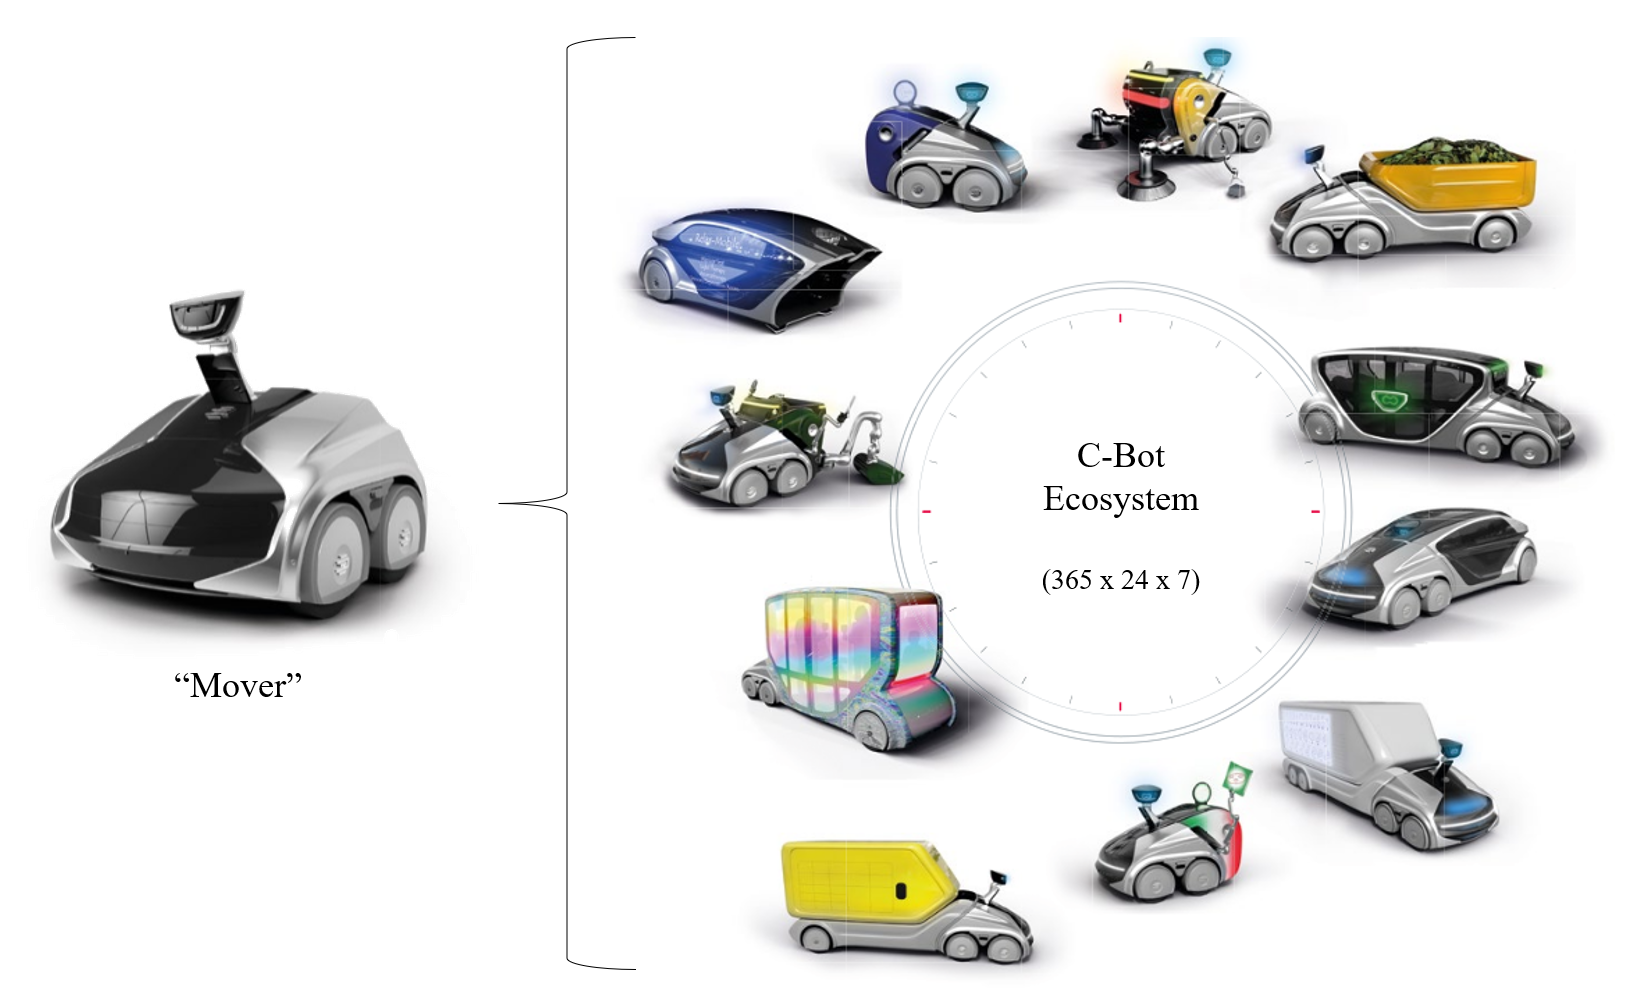
\includegraphics[width=1\textwidth]{resources/images/020-introduction/Introduction_context_C-Bot.png}
        \smallcaption{Source: Author, "adapted from" the original confidential source}
        \label{fig:introduction_C-Bot_ecosystem}
\end{figure} 

In the background, and as part of the C-Bot project, the control system optimizes route planning and the utilization of the C-Bots in continuous 24-hour operation. Users can conveniently input their requests into the system, whether it be the user requesting transportation to the next stop via app, the store owner planning the delivery of new products for the following day, or the municipal vehicle organizing overnight waste removal. This can massively reduce the number of vehicles in city centers, make parking spots available for other uses, and alleviate traffic jams through consistent coordination. All of this makes a significant contribution to the concept of "shared space" traffic, where all \textbf{road users coexist on an equal footing}, and to a smart, sustainable, and livable city.

The project is currently in its third phase, as shown in Figure \ref{fig:introduction_C-Bot_roadmap}, where development partners will explore challenges and possible solutions for core elements of the planned ecosystem: \textbf{automated driving functions}, networking and data exchange, \gls{hci}, \textbf{acceptance and trust}, integrated order management, identification and realization of potential economic and technical optimization in operation, and many more secondary elements\footnote{Citations were omitted due to the disclaimed blocking and restriction notice.}. 

\begin{figure}[htbp]
    \raggedright
        \caption{Roadmap of the C-Bot development, since its original concept presented in 2019 until its fully implementation in public areas in 2030.}
        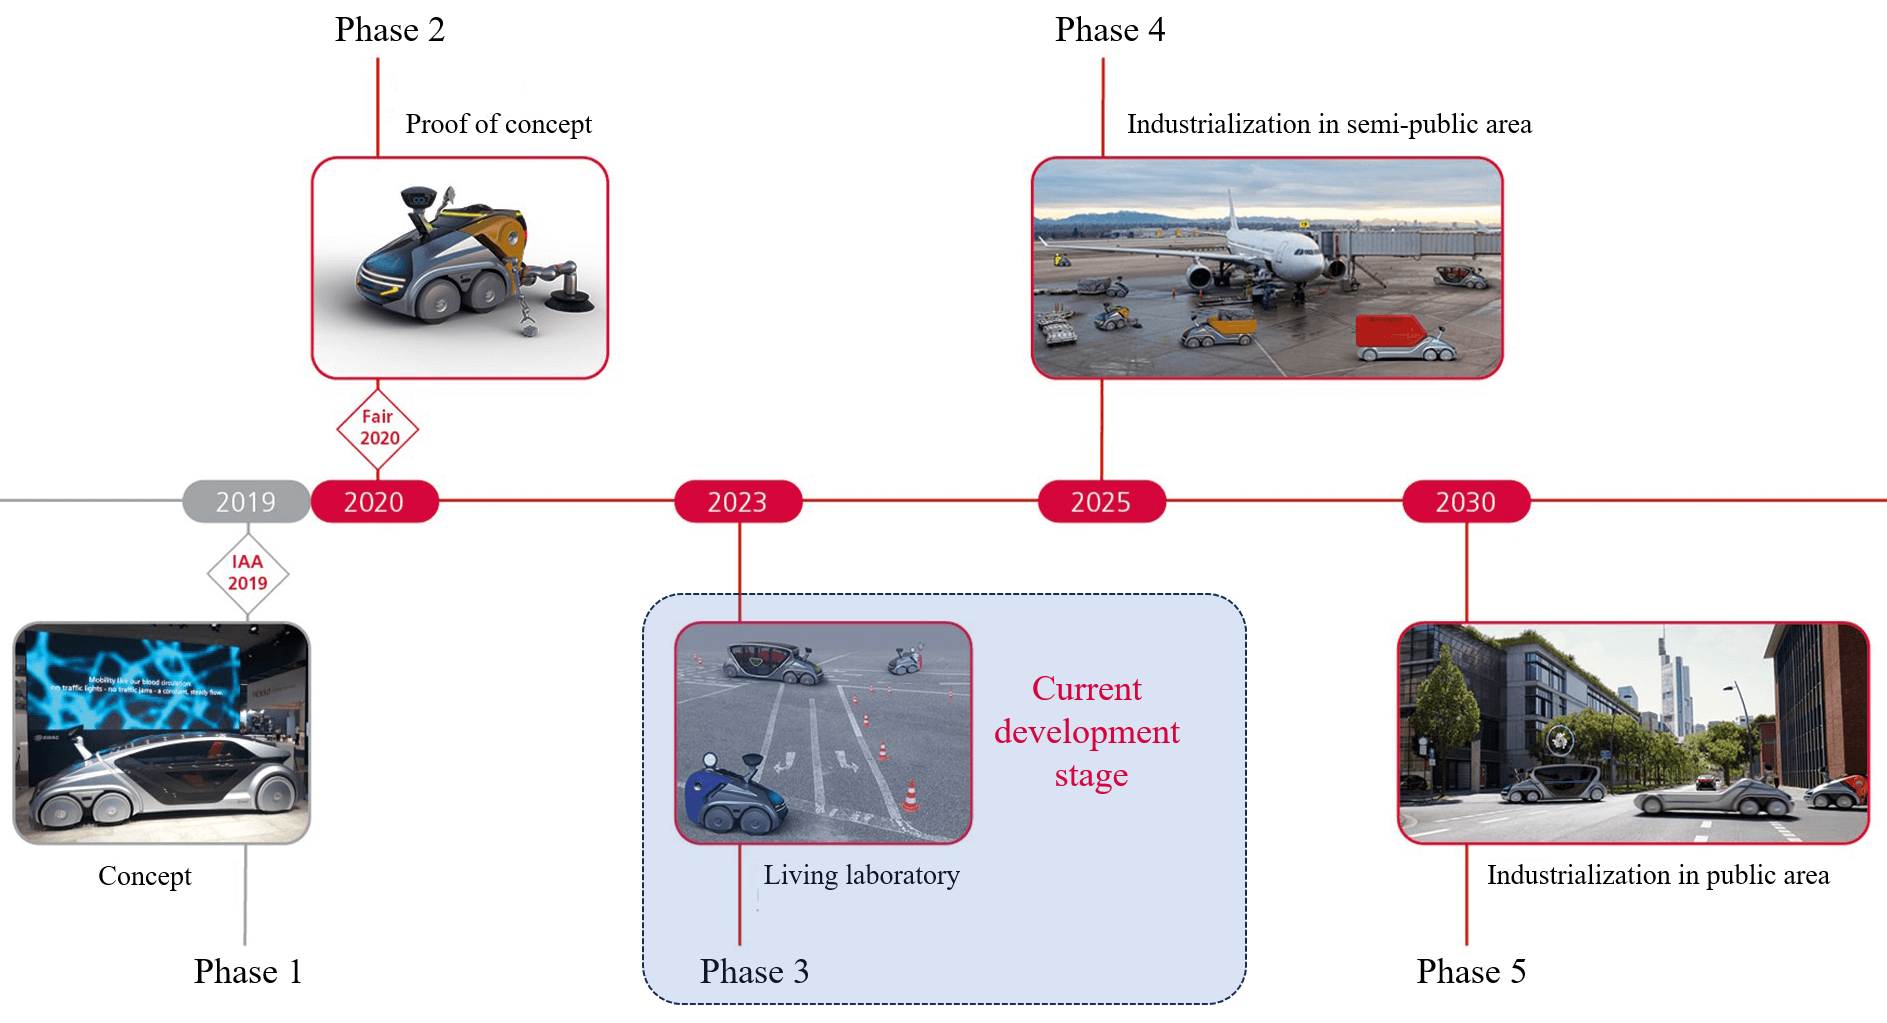
\includegraphics[width=1\textwidth]{resources/images/020-introduction/Introduction_context_C-Bot_roadmap.png}
        \smallcaption{Source: Author, "adapted from" the original confidential source}
        \label{fig:introduction_C-Bot_roadmap}
\end{figure} 

In this phase, the C-Bots are equipped with speech recognition capabilities enabling \gls{hci} with the end-users, however, as in all other autonomous vehicles identified until this publication, \gls{esr} is not yet implemented. Throughout several meetings with the project product owner and the technical staff, the feature of the \gls{esr} was ranked as "important" in the product backlog and it shall be integrated in the next milestone (Phase 4), primarily to confirm its implementation feasibility in the vehicle \gls{ee} and its relevance as a feature itself.


\section{OBJECTIVE}
\label{sec:introduction_objective}

The objective of this study is to develop and implement an \gls{esr} algorithm in embedded systems for autonomous vehicles ranging from level 2 to level 5. This can be achieved by investigating existing sound recognition algorithms, analyzing their performance, and selecting the most suitable ones for real-time embedded implementation.


\subsection{General objective}
\label{subsec:objectives_general}

As a general objective, this study intends to investigate whether it's feasible to enhance the perception capabilities of autonomous vehicles by enabling them to recognize and classify environmental sounds, merging the output into the sensor fusion network to produce specific responses from the vehicle \gls{ee} architecture in due time. If the feasibility is confirmed, this study may contribute to improving their safety, decision-making, and overall autonomy. 

Considering the context presented in section \ref{sec:introduction_context}, and the fact that the C-Bot hardware construction is under development in a foreign country, an alternative approach to validate this study is proposed using as context, a regular passenger vehicle, with the \gls{esr} algorithms embedded in a high-end general-purpose platform, a separated microphone array to emulate the audio processing capabilities of the vehicle control unit and the same microphone utilized in the vehicle for speech recognition tasks.

\subsection{Specific objectives}
\label{subsec:objectives_specifics}

To achieve the general objective, this section outlines the specific objectives of this study:

\begin{itemize}
    \item Dataset benchmarking to confirm the classifiers' accuracy:
    \begin{itemize}
        \item Establish the benchmark datasets consisting of diverse environmental sounds that will be used to evaluate the accuracy and performance of the implemented classifiers;
        \item Implement and train different classifiers utilizing the benchmark datasets;
        \item Assess the accuracy of the classifiers by comparing their results against known ground truth labels (validation sets) and the literature results.
    \end{itemize}
    \item Construction of a new dataset tailored for environmental sounds in the  context of autonomous vehicles:
    \begin{itemize}
        \item Define the relevant classes within the benchmark datasets that are relevant for this study, considering also the alternative approach proposed in the general objectives;
        % \item Compare the classes of the tailored dataset with YAMNet, a model developed by Google that is specifically designed for sound classification tasks.
    \end{itemize}
    \item Training and evaluating the classifiers on a notebook and in an embedded device:
    \begin{itemize}
        \item Implement and train the classifiers on a high-performance notebook computer using both benchmark and tailored datasets;
        \item Evaluate the classifiers' performance in terms of accuracy, computational efficiency, and memory requirements;
        \item Deploy the best-performing classifier to an embedded device, specifically a Raspberry Pi, and assess its performance in terms of accuracy and real-time processing capabilities.
    \end{itemize}
    \item Evaluating the best classifier in the context of a regular passenger vehicle:
    \begin{itemize}
        \item Prepare the Raspberry Pi model to receive a microphone array and a microphonic sensor;
        \item Evaluate the classifier's performance in the realistic context of a passenger vehicle, taking into consideration factors such as background noise, varying environmental conditions, and real-time response requirements;
        \item Assess the classifier's ability to contribute to the enhancement of the vehicle's safety, decision-making, and overall autonomy. As ramification of this study, assess the contribution of the classifier in the context of a regular passenger vehicle.
    \end{itemize}
\end{itemize}


\section{ORGANIZATION}
\label{sec:introduction_organization}

The organization of this study is structured into four chapters. In chapter \ref{chp:frmwk} , the theoretical framework of the main concepts is outlined. Initially, the concepts and definitions related to audio processing are presented in section \ref{sec:frmwk_audio_fund}. Microphones and their automotive applications are explained in section \ref{sec:frmwk_microphones}, while section \ref{sec:frmwk_machine_learning} highlights the machine learning and ensemble methods implemented in the classifiers, followed by section \ref{sec:frmwk_neural_networks} that presents the same idea, but for neural networks. %Section \ref{sec:frmwk_classification_metrics} outlines the metrics involved in classification tasks while Section \ref{sec:frmwk_environmental_sound_classification} is more specific and highlights the definition of environmental sound classification and trained networks available.
The chapter ends on section \ref{sec:frmwk_electronic_control_unit} where the hardware platforms in the automotive industry are presented, including the proposal utilized in the experiments of this study.

Chapter \ref{chp:rel} addresses the state of the art in the recognition of environmental sound, where various concepts and works related to the proposed research are presented and discussed.

Chapter \ref{chp:methods} focuses on the methods and materials employed in this study, encompassing section \ref{sec:methods_HWSW} where the hardware and software aspects are discussed in detail. This section provides an overview of the specific systems and tools utilized for the implementation and execution of the \gls{esr} algorithms. Section \ref{sec:methods_dataset} pertains to the datasets used for training, evaluation and benchmarking purposes, outlining their content, the classifiers and features utilized for sound classification and its metrics. Normalization techniques applied to preprocess the audio data are described in section \ref{sec:methods_normalization}. It elaborates on the normalization methods used to ensure consistency and optimal performance during the subsequent stages of this study. In section \ref{sec:methods_augmentation}, the augmentation techniques employed to enhance the dataset are explained, providing insights into the methods used to artificially increase the size and diversity of the dataset. Section \ref{sec:methods_feature_extraction} delves into the feature extraction process, detailing the techniques employed to extract relevant acoustic features from the audio data, taking into consideration the specific requirements for \gls{esr}. The training procedures followed for the classifiers are discussed in section \ref{sec:methods_training_classifiers}. This section outlines the steps taken to train the machine learning, ensemble and neural network models, including the optimization of hyperparameters. Finally, section \ref{sec:methods_evaluation} addresses the evaluation procedures utilized to assess the performance of the implemented classifiers.

Chapter \ref{chp:results} presents the results of the conducted experiments encompassing section \ref{sec:results_metrics} that focuses on the evaluation metrics used, including accuracy, processing memory, allocation memory and response time. While section \ref{sec:results_training_classification_flow} outlines the results in the training and classification flow and the results of the evaluation flow into a regular passenger vehicle.

At last, chapter \ref{chp:conclusion} brings the conclusion and future work within the context of \gls{esr} for autonomous vehicles and regular passenger vehicles.


\section{HYPOTHESES}
\label{sec:introduction_hypotheses}

The purpose of this chapter is to enumerate all conceivable hypotheses that may arise from the present study, whether they pertain to practical applications or scientific advancements. The specific articulation of how these hypotheses will be incorporated into the dissertation remains to be determined.

\begin{table}[ht!]
    \caption[List of alternative hypotheses $H_a$ defined during the study development ]{List of alternative hypotheses $H_a$, potential application or contribution, and current status of its implementation on this study.}
    \label{table:hypotheses_list_ha}
    \centering
    \begin{tabular}{p{1.7cm}|p{6.5cm}|p{6.5cm}}
        \Xhline{2\arrayrulewidth} 
        \rowcolor{lightgray}
        \textbf{Id} & \textbf{Description} & \textbf{Application or contribution} \\
        $H_1$ & 
        \gls{esr} is performed in milliseconds, perhaps even seconds, before other types of object detection (cameras, radars, and sensors) & 
        Other sensors can be set to higher levels of accuracy based on \gls{esr} outputs or be complemented by sensor fusion techniques. \\
        \hline
        \rowcolor{gray!20} Status $H_1$ & \multicolumn{2}{c}{\parbox{13.4cm}{\textbf{Alternative $H_a$}. \textcite{Veeraraghavan2020} confirmed by  Simulink simulations the feasible of an acoustic controlled driving system level 3. Initial findings of \textcite{Yin2023} also confirmed a suitable response time (Section \ref{chp:rel}) }} \\       
        \hline \hline
%        $H_4$ & 
%        \gls{esr} has potential applications also in regular passenger cars, without any additional costs on hardware or devices. & 
%        Adding code lines in the current \gls{vcu} or infotainment \gls{ecu} and broadcast messages or warnings to the driver.\\
%        \hline
%        \rowcolor{yellow} Status $H_4$ & \multicolumn{2}{c}{\parbox{13.4cm}{\textbf{Null ($H_0$) or alternative $H_a$}. Under investigation...}} \\       
%        \hline \hline
        $H_2$ & 
        Driving a vehicle requires: sight or vision, touch or somatosensation, and hearing or audition. To this publication, autonomous vehicles have been neglecting the last one, it’s plausible to state that \gls{esr} integrated in the vehicle \gls{ee} architecture will improve its drivability experience. & 
        Safer conditions to the vehicle occupants and overall better user experience.\\
        \hline
        \rowcolor{gray!20} Status $H_2$ & \multicolumn{2}{c}{\parbox{13.4cm}{\textbf{Alternative $H_a$}. To this point, this study concludes that the integration of \gls{esr} in autonomous vehicles seems logical and feasible, however, there is no empirical evidence of improvement in the drivability experience.}} \\       
        \Xhline{2\arrayrulewidth}
    \end{tabular}
    \smallcaption{Source: Author}
\end{table}


\begin{table}[ht!]
    \caption[List of null hypotheses $H_0$ defined during the study development ]{List of null hypotheses $H_0$, potential application or contribution, and current status of its implementation on this study.}
    \label{table:hypotheses_list_h0}
    \centering
    \begin{tabular}{p{1.7cm}|p{6.5cm}|p{6.5cm}}
        \Xhline{2\arrayrulewidth} 
        \rowcolor{lightgray}
        \textbf{Id} & \textbf{Description} & \textbf{Application or contribution} \\
        \hline
        $H_3$ &
        A regular passenger car microphone has auditory sensitivity higher or equivalent than human ears. &
        If confirmed, there will be no need of special acoustic devices to identify specific sounds. \\
        \hline
        \rowcolor{gray!20} Status $H_3$ & \multicolumn{2}{c}{\parbox{13.4cm}{\textbf{Null ($H_0$)}. However, it is imperative to note that automotive microphones do exhibit sufficient attributes capable of detecting a substantial range of acoustic events. This inference imparts significant technological insights regarding the use of automotive microphones in environmental sound recognition (Section \ref{subsec:microphones_conclusion}).}} \\
        \hline \hline
        $H_4$ & 
        \gls{esr} will not improve decision-making algorithms of autonomous vehicles by merging its output into the sensor fusion network of the vehicle. & 
        If null, faster and more accurate information can be transmitted to the driver. \\
        \hline
        \rowcolor{gray!20} Status $H_4$ & \multicolumn{2}{c}{\parbox{13.4cm}{\textbf{Null $H_0$}. One government funding project \cite{ISPOT2020} is exploring this topic, and in the private industry, one prototype already implemented audio sensor fusion \cite{WAYMO2023}, (Section \ref{chp:rel})}} \\        
        \hline \hline
%        $H_4$ & 
%        \gls{esr} has potential applications also in regular passenger cars, without any additional costs on hardware or devices. & 
%        Adding code lines in the current \gls{vcu} or infotainment \gls{ecu} and broadcast messages or warnings to the driver.\\
%        \hline
%        \rowcolor{yellow} Status $H_4$ & \multicolumn{2}{c}{\parbox{13.4cm}{\textbf{Null ($H_0$) or alternative $H_a$}. Under investigation...}} \\       
%        \hline \hline
        $H_5$ & 
        It’s not possible to identify an object trajectory through \gls{esr} in a time frame (sound vector). & 
        If null, different \gls{esr} outputs to the driver depending whether the identified sound is moving away or approaching the vehicle.\\
        \hline
        \rowcolor{gray!20} Status $H_5$ & \multicolumn{2}{c}{\parbox{13.4cm}{\textbf{Null ($H_0$)}. Using external microphone array \cite{Marchegiani2022} and \cite{Sun2021}, and with internal microphone array \cite{Shabtai2019}, (Section \ref{chp:rel}) }} \\           
        \Xhline{2\arrayrulewidth}
    \end{tabular}
    \smallcaption{Source: Author}
\end{table}

